%% ==========================================================================
%% GENERATED by paper/ejp/tools/make_aps_revtex.py from paper/ejp/jc_beyond_linear.tex.
%% Do not edit this file: edit the source and run the script again.
%% RESEARCH CUT: without the teaching section, the exercises and the sentences addressed to
%% students (CUT_* in the script).
%% Build: tectonic jc_beyond_linear_aps_research.tex
%% ==========================================================================
\documentclass[%
 reprint,
 amsmath,amssymb,
 aps,
 floatfix,
]{revtex4-2}

\usepackage{graphicx}
\graphicspath{{../figures/}{../../figures/}}
\usepackage[colorlinks=true,linkcolor=blue,citecolor=blue,urlcolor=blue]{hyperref}
\newcommand{\nbar}{\bar{n}}
\newcommand{\ket}[1]{|#1\rangle}
\newcommand{\bra}[1]{\langle #1|}
\newcommand{\braket}[2]{\langle #1|#2\rangle}

\begin{document}

\title{Rotation and shear in the Jaynes--Cummings model: What the curvature of the Rabi spectrum does to revivals, cat states, and entanglement}

\author{Nguyen Khoi Nguyen}
\email{nknguyen@bu.edu}  % confirm the address to be published
\affiliation{Department of Electrical and Computer Engineering, Boston University, Boston, Massachusetts 02215, USA}
\affiliation{Department of Physics, Boston University, Boston, Massachusetts 02215, USA}

\date{\today}

\begin{abstract}
The textbook account of collapse and revival in the Jaynes--Cummings model expands the Rabi frequencies $2g\sqrt{n+1}$ (coupling $g$) to first order about the mean photon number $\nbar$. Gea-Banacloche carried the expansion to second order in 1991. We give that order a geometric reading, extend the expansion to order $1/\nbar$, and test every result against the exact solution. To first order the two components of the cavity field rotate in opposite directions in phase space, by the angle $\varphi = gt/2\sqrt{\nbar}$. To second order each is sheared by an amount equal to its rotation angle, which is the origin of its known squeezing. The overlap of two sheared Gaussians recovers the known height $(1+\pi^2k^2)^{-1/4}$ of the $k$th revival and gives closed forms that are, to our knowledge, new: the amplitude and phase of a revival of the photon-number parity at half the revival time, and the limiting Wigner negativity of the cat state formed then. The fidelity of that state with an ideal cat state, $(1+\pi^2/16)^{-1/2} = 0.786$, does not improve with $\nbar$. The next order gives the residual atom--field entanglement and $1/\nbar$ corrections to the revival amplitudes. We show where the expansion fails and document the limits of the numerical methods.
\end{abstract}

\keywords{Jaynes--Cummings model, collapse and revival, Schr\"{o}dinger cat state, squeezing, Wigner function, asymptotic expansion}

\maketitle

\section{Introduction}
\label{sec:intro}

The Jaynes--Cummings (JC) model~\cite{jaynes1963}, a two-level atom exchanging one quantum at a time with a single cavity mode, is the simplest setting in which the quantized field does something a classical field cannot. If the field starts in a coherent state, the Rabi oscillations of the atom collapse and, much later, revive~\cite{eberly1980}. The standard explanation~\cite{gerry2004, haroche2006} is brief. The $n$-photon term of the state oscillates at the Rabi frequency $2g\sqrt{n+1}$, where $g$ is the coupling; the set of these frequencies is the Rabi spectrum. Linearizing it about the mean photon number $\nbar$ shows that the terms of different $n$ dephase in a time of order $1/g$ and, because $n$ is an integer, rephase at the revival time $t_r = 2\pi\sqrt{\nbar}/g$.

A simulation shows a good deal that this argument does not explain. The revival is not complete: for $\nbar = 10$ the oscillations return to about half their initial amplitude. Halfway to the revival the cavity field is in a Schr\"{o}dinger cat state~\cite{gea-banacloche1990, gea-banacloche1991, buzek1992}, but its fidelity with an ideal cat state is 0.78 for $\nbar = 10$ and never exceeds 0.79, however large $\nbar$ is made. The photon-number distribution at that moment is a comb of odd numbers for $\nbar = 10$ and of even numbers for $\nbar = 9$. The atom and field are then nearly, but not exactly, disentangled~\cite{gea-banacloche1990, phoenix1991}. These values are reproducible, which suggests a simple origin.

The origin is the curvature of the square root. Keeping the next term of its expansion accounts for the first three of these observations in closed form, and the order after it for the fourth. The organizing picture is geometric (Fig.~\ref{fig:wigner}): the linear term \emph{rotates} the two components of the field in phase space, and the quadratic term, which makes the angular velocity depend on photon number, \emph{shears} them, in the same way that differential rotation shears a galaxy or a planetary ring. The shear equals the rotation angle, and the constants above are overlaps of two sheared Gaussians. The order after that gives $1/\nbar$ corrections that we compute and check.

Much of this physics is established; we state here which parts. The collapse and revival envelopes were derived by Eberly and co-workers~\cite{eberly1980, narozhny1981}, recast with the Poisson summation formula by Fleischhauer and Schleich~\cite{fleischhauer1993}, and appear in explicit form in Refs.~\cite{feranchuk2009, pavlik2024}. The two-component structure of the state, the disentanglement at $t_r/2$, and the cat state are due to Gea-Banacloche~\cite{gea-banacloche1990, gea-banacloche1991} and to Phoenix and Knight~\cite{phoenix1991, phoenix1988}, with phase-space pictures in Refs.~\cite{gea-banacloche1991, buzek1992, eiselt1991, larson2021, knight2024}. Gea-Banacloche also carried the expansion to second order: Appendix~B of Ref.~\cite{gea-banacloche1991} gives the state with the quadratic phase, the quadrature variances of each component [his Eqs.~(B11)--(B13), equivalent to our Eq.~(\ref{eq:shear})], its $Q$ function, and the value 0.55 for the overlap of the two components at the first revival, and it likens the components to the states produced by a Kerr medium. The same quadratic phase was identified as the source of the ``phase spreading'' of the components in the analysis of experiments~\cite{auffeves2003, bild2023}. Squeezing in the model has its own literature~\cite{meystre1982, kuklinski1988, woods1993}. The decay of the purity between collapse and revival was found in Ref.~\cite{gea-banacloche1992}, and the Bloch vector of the atom there is given in Ref.~\cite{kennedy2010}. The oscillation of the photon-number parity near $t_r/2$ was studied numerically~\cite{knight2024, birrittella2015}, and its leading-order value was given in connection with experiment~\cite{assemat2019}. The model with cavity loss was analyzed in Refs.~\cite{gea-banacloche1993, meunier2006}. A fidelity of 0.79 between the half-revival field and a cat state was found numerically in Ref.~\cite{munhoz2005}.

What we add is a geometric reading of the second order, namely that each component is sheared by an amount equal to its rotation angle, which is implicit in the variances of Ref.~\cite{gea-banacloche1991}; one elementary derivation that ties these results together; and several closed forms that we have not found in the literature: the amplitude and phase of the parity revival, the limiting Wigner negativity, the complete $1/\nbar$ term of the purity, and the $1/\nbar$ correction to the revival amplitudes. We also point out that the overlap of a component with a coherent state, which follows from the $Q$ function of Ref.~\cite{gea-banacloche1991}, is the fidelity of the half-revival state with an ideal cat state and does not improve with $\nbar$, contrary to a common statement~\cite{larson2021}. Each of these can be tested against the exact solution to three or four digits. We also give an account of how well the expansion and the numerics work, which we regard as part of the physics: Sec.~\ref{sec:numerics} and the Supplemental Material~\cite{supplement} treat the simulation as an experiment with its own systematic errors.

Section~\ref{sec:model} states the exact solution, Sec.~\ref{sec:orders} sets out the expansion, and Secs.~\ref{sec:rotation}--\ref{sec:next} take its orders one at a time. Section~\ref{sec:numerics} tests the results and discusses the numerical methods, and Sec.~\ref{sec:loss} adds cavity loss.

\section{The model and its exact solution}
\label{sec:model}

On resonance and in the interaction picture the JC Hamiltonian is
\begin{equation}
H = \hbar g\left(a^\dagger\sigma^- + a\,\sigma^+\right),
\label{eq:H}
\end{equation}
where $a$ annihilates a cavity photon, $\hat{n} = a^\dagger a$ is the photon number, $\sigma^\pm$ raise and lower the atom between $\ket{g}$ and $\ket{e}$, and $g$ is the coupling. The Hamiltonian couples $\ket{e,n}$ only to $\ket{g,n+1}$, so for the initial state $\ket{e}\otimes\ket{\alpha}$, with $\ket{\alpha}$ a coherent state of real amplitude $\alpha = \sqrt{\nbar}$, the state at time $t$ is known exactly:
\begin{equation}
\begin{aligned}
\ket{\psi(t)} &= \sum_{n=0}^{\infty} c_n\big[\cos\theta_n\,\ket{e,n} - i\sin\theta_n\,\ket{g,n+1}\big],\\
\theta_n &= gt\sqrt{n+1},\qquad c_n = e^{-\nbar/2}\frac{\alpha^n}{\sqrt{n!}}.
\end{aligned}
\label{eq:exact}
\end{equation}
The photon-number weights $p_n = c_n^2$ are Poissonian, with mean and variance $\nbar$. All the results for the lossless model follow from Eq.~(\ref{eq:exact}), and our numerical tests of them use it directly.

Writing the cosine and sine as exponentials splits the state into two parts, one for each sign of the phase. Following Gea-Banacloche~\cite{gea-banacloche1991} we call the corresponding field states
\begin{equation}
\ket{\Phi_\pm(t)} = e^{\pm i gt\sqrt{\hat{n}+1}}\ket{\alpha} = \sum_n c_n e^{\pm i\theta_n}\ket{n},
\label{eq:branches}
\end{equation}
because two familiar observables are then overlaps of these two states. The atomic inversion is $\langle\sigma_z\rangle = \sum_n p_n\cos 2\theta_n$, and a short calculation gives the photon-number parity $\langle(-1)^{\hat n}\rangle = \sum_n p_n(-1)^n\cos 2\theta_n$, so that
\begin{equation}
\begin{aligned}
\langle\sigma_z\rangle &= \mathrm{Re}\,\braket{\Phi_-}{\Phi_+},\\
\langle(-1)^{\hat{n}}\rangle &= \mathrm{Re}\,\bra{\Phi_-}(-1)^{\hat{n}}\ket{\Phi_+}.
\end{aligned}
\label{eq:overlaps}
\end{equation}
The operator $(-1)^{\hat n}$ rotates phase space by $\pi$, that is, it reflects every point through the origin. Equation~(\ref{eq:overlaps}) therefore says: the inversion measures how much the two field components overlap~\cite{gea-banacloche1991, auffeves2003}, and the parity measures how much one overlaps with the reflection of the other. These two identities are exact.

We describe the field in the phase space $(x,p)$ with $a = (x+ip)/\sqrt{2}$, in which the vacuum has variance $1/2$ in each direction and $\ket{\alpha}$ sits at distance $\sqrt{2\nbar}$ from the origin, and we use the Wigner function $W(x,p)$ and its negativity $\delta = \int|W|\,dx\,dp - 1$~\cite{kenfack2004}.

\section{Expanding the Rabi spectrum}
\label{sec:orders}

Put $n = \nbar + \delta n$. The Poisson distribution confines $\delta n$ to a range of order $\sqrt{\nbar}$, so for large $\nbar$ we may expand
\begin{equation}
\begin{aligned}
\theta_n &\simeq gt\sqrt{\nbar}\,\Big[1 + \frac{\delta n}{2\nbar} - \frac{\delta n^2}{8\nbar^2} + \frac{\delta n^3}{16\nbar^3} - \dots\Big]\\
&= gt\sqrt{\nbar} + \varphi\,\delta n - \frac{\varphi\,\delta n^2}{4\nbar} + \frac{\varphi\,\delta n^3}{8\nbar^2} - \dots,
\end{aligned}
\label{eq:expansion}
\end{equation}
where $\varphi \equiv gt/2\sqrt{\nbar}$. (Here $n+1$ has been replaced by $n$. This drops a constant $\varphi$ from $\theta_n$, which is of order one and fixes the sign of Eq.~(\ref{eq:parity}), and terms of relative order $\nbar^{-1/2}$, which move the center of the $k$th revival from $kt_r$ to about $2\pi k\sqrt{\nbar+1}/g$; the amplitudes at $t = kt_r$ change only at relative order $1/\nbar$. All of this is kept in Sec.~\ref{sec:next}, in the Supplemental Material, and in the figures.) The single parameter $\varphi$ measures time in the natural unit: the revival time corresponds to $\varphi = \pi$. For $\varphi$ of order one, with $\delta n \sim \sqrt{\nbar}$, the successive terms of Eq.~(\ref{eq:expansion}) are of order $\nbar$, $\sqrt{\nbar}$, $1$, $\nbar^{-1/2}$. Table~\ref{tab:orders} lists what each does. The textbook treatment keeps orders 0 and 1. The order-2 term is not small: it is of order one for any $\nbar$, as noted in Refs.~\cite{gea-banacloche1991, auffeves2003}, which is why its consequences are numbers that do not depend on $\nbar$ at all.

\begin{table*}[t]
\caption{The orders of the expansion in Eq.~(\ref{eq:expansion}) at times $t \sim \sqrt{\nbar}/g$, with $\delta n = n - \nbar \sim \sqrt{\nbar}$.}
\label{tab:orders}
\begin{ruledtabular}
\begin{tabular}{clcl}
Order & Term & Size & Effect on a field component \\
\hline
0 & $gt\sqrt{\nbar}$ & $\nbar$ & common phase: the Rabi oscillation itself \\
1 & $\varphi\,\delta n$ & $\sqrt{\nbar}$ & rotation by the angle $\varphi$ (collapse, revival) \\
2 & $-\varphi\,\delta n^2/4\nbar$ & $1$ & shear $s = \varphi$: squeezing, imperfect revivals \\
3 & $\varphi\,\delta n^3/8\nbar^2$ & $\nbar^{-1/2}$ & skewing; changes the amplitudes at order $1/\nbar$ \\
\end{tabular}
\end{ruledtabular}
\end{table*}

\section{First order: two components that rotate}
\label{sec:rotation}

Keep the first two terms of Eq.~(\ref{eq:expansion}). Since $e^{\pm i\varphi\hat{n}}\ket{\alpha} = \ket{\alpha e^{\pm i\varphi}}$, the two field states are coherent states that rotate in opposite directions:
\begin{equation}
\ket{\Phi_\pm(t)} \simeq e^{\pm i\vartheta}\ket{\alpha e^{\pm i\varphi}},
\label{eq:rotation}
\end{equation}
with $\vartheta = gt\sqrt{\nbar}/2$ a phase that does not depend on $n$. Their angular velocity is $g/2\sqrt{\nbar}$. By Eq.~(\ref{eq:overlaps}) the envelope of the inversion is their overlap, $|\braket{\alpha e^{-i\varphi}}{\alpha e^{i\varphi}}| = \exp(-2\nbar\sin^2\varphi)$. For small $\varphi$ this is $\exp(-g^2t^2/2)$: the oscillations collapse as soon as the two components, each of vacuum size, have separated, which takes a time $1/g$ whatever the radius $\sqrt{2\nbar}$ of the circle. The overlap returns to unity when the components meet again on the far side, at $\varphi = \pi$, that is, at the revival time~\cite{eberly1980, gea-banacloche1991}.

The same order describes the atom. Collecting the terms of Eq.~(\ref{eq:exact}) that multiply each field state, and using the fact that shifting $n$ by one changes $\theta_n$ by $\varphi$ to this order, gives
\begin{equation}
\begin{aligned}
\ket{\psi(t)} &\simeq \frac{1}{\sqrt{2}}\Big[\ket{\Phi_-}\ket{\chi_-} + \ket{\Phi_+}\ket{\chi_+}\Big],\\
\ket{\chi_\mp} &= \frac{1}{\sqrt{2}}\left(\ket{e} \pm e^{\pm i\varphi}\ket{g}\right).
\end{aligned}
\label{eq:twobranch}
\end{equation}
This is the two-branch form found by Gea-Banacloche~\cite{gea-banacloche1990, gea-banacloche1991}. While the two field components still overlap, Eq.~(\ref{eq:twobranch}) is not a Schmidt decomposition. Once they have separated it is one, up to the overlap of the two atomic states, $|\braket{\chi_-}{\chi_+}| = |\sin\varphi|$. The reduced atomic state then has eigenvalues $\lambda_\pm = \tfrac{1}{2}(1\pm|\sin\varphi|)$, so the purity $\mathcal{P} = \mathrm{Tr}\,\rho^2$ of either reduced state $\rho$ and the entanglement entropy $S = -\mathrm{Tr}\,\rho\log_2\rho$ are
\begin{equation}
\mathcal{P}(t) = 1 - \tfrac{1}{2}\cos^2\varphi,\qquad
S(t) = h(\lambda_+),
\label{eq:skeleton}
\end{equation}
where $h(\lambda) = -\lambda\log_2\lambda-(1-\lambda)\log_2(1-\lambda)$ is the binary entropy. Just after the collapse, where $\varphi \approx 0$, the two atomic states are orthogonal, $\mathcal{P} = 1/2$, and $S = 1$~bit: the reduced field is an equal \emph{mixture} of the two components. At $\varphi = \pi/2$, half the revival time, the two atomic states coincide, the state factorizes, and the field is left in the superposition $(\ket{\Phi_-}+\ket{\Phi_+})/\sqrt{2}$ of two components on opposite sides of phase space: a Schr\"{o}dinger cat state, formed at the moment of \emph{least} entanglement. Equation~(\ref{eq:skeleton}) gives the slowly varying part of the purity and entropy curves between collapse and revival; Sec.~\ref{sec:next} compares it with the exact curves.

At this order the revival would be perfect, the cat would be an ideal superposition of two coherent states, and the atom would disentangle completely. None of these statements holds exactly; Secs.~\ref{sec:shear} and \ref{sec:next} quantify the departures.

\begin{figure*}[t]
\centering
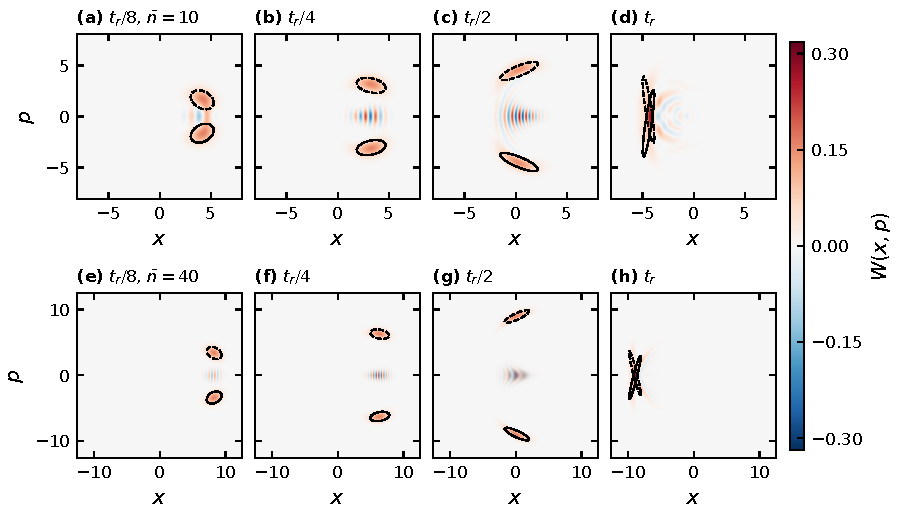
\includegraphics[width=6in]{fig_wigner_shear.pdf}
\caption{Wigner function of the reduced cavity field (exact) at $t = t_r/8$, $t_r/4$, $t_r/2$, and $t_r$ (left to right), for $\nbar = 10$ (a)--(d) and $\nbar = 40$ (e)--(h), with the prediction of the rotation-and-shear picture drawn on top. Each curve is the $1/e$ contour of a Gaussian centered at distance $\sqrt{2\nbar}$ from the origin, sheared according to Eq.~(\ref{eq:shear}), with no adjustable parameter: the solid curve is the component at angle $-\varphi'$ and the dashed curve the one at $+\varphi'$, where $\varphi' = gt/2\sqrt{\nbar+1}$ keeps the $n+1$ of the exact phases ($\varphi' \to \varphi$ for large $\nbar$). The fringes between the components are their interference; for $\nbar = 40$ they are too fine to be resolved at this scale. At $t_r/2$ the components are opposite each other (cat state); at $t_r$ they almost coincide in position but are sheared in opposite senses, which is why the revival is incomplete. The residual mismatch at $\nbar = 10$ is the bending of the components along the circle, an effect of relative order $\nbar^{-1/2}$ that is present already for a purely quadratic phase (a function of $\hat n$ moves points along arcs, not along the tangent).}
\label{fig:wigner}
\end{figure*}

\section{Second order: differential rotation shears the components}
\label{sec:shear}

The angular velocity $g/2\sqrt{n}$ of a component depends on its photon number, that is, on its radius in phase space: the outer part of each component lags and the inner part leads. After a time $t$ a point whose radial coordinate differs from the mean by $\delta R$ has been displaced tangentially by $-\varphi\,\delta R$. This is a shear, and its magnitude is the rotation angle itself:
\begin{equation}
s(t) = \varphi(t) = \frac{gt}{2\sqrt{\nbar}}.
\label{eq:s}
\end{equation}
It is exactly what the quadratic term of Eq.~(\ref{eq:expansion}) does, because $\delta n$ is $\sqrt{2\nbar}$ times the radial coordinate, so that $\varphi\,\delta n^2/4\nbar$ is a quadratic form in that coordinate (Sec.~S1 of the Supplemental Material). In coordinates (radial, tangential) the covariance matrix of a component changes from that of the vacuum, $\tfrac{1}{2}I$ with $I$ the $2\times2$ unit matrix, to
\begin{equation}
V(\pm s) = \frac{1}{2}\begin{pmatrix} 1 & \pm s \\ \pm s & 1+s^2 \end{pmatrix},
\label{eq:shear}
\end{equation}
the two signs belonging to the two components. The determinant is unchanged, so each component remains a minimum-uncertainty Gaussian: a squeezed coherent state with squeezing parameter $r$ given by $\sinh r = s/2$. The eigenvalues of $V(s)$ are the quadrature variances obtained by Gea-Banacloche~\cite{gea-banacloche1991}; Eq.~(\ref{eq:shear}) states his result as a shear. Figure~\ref{fig:wigner} compares this prediction with the exact Wigner function.

Most of the consequences follow from one fact. Two pure Gaussian states with a common center and covariance matrices $V_1$, $V_2$ have squared overlap $[\det(V_1+V_2)]^{-1/2}$. In photon-number language the same statement is the Gaussian integral
\begin{equation}
\begin{gathered}
\big\langle e^{-i\mu\,\delta n^2}\big\rangle = (1+2i\mu\nbar)^{-1/2}\\
\text{for $\delta n$ Gaussian with variance $\nbar$.}
\end{gathered}
\label{eq:lemma}
\end{equation}

\textit{Incomplete revivals.} At the $k$th revival, $\varphi = k\pi$, the two components are in the same place but sheared by $+k\pi$ and $-k\pi$. From Eq.~(\ref{eq:shear}), $\det[V(s)+V(-s)] = 1+s^2$, so the envelope of the inversion returns only to
\begin{equation}
\begin{aligned}
&\big|\braket{\Phi_-}{\Phi_+}\big|_{t = kt_r} \simeq (1+\pi^2k^2)^{-1/4}\\
&\qquad = 0.551,\ 0.396,\ \dots\quad\text{for } k = 1,\ 2,\ \dots.
\end{aligned}
\label{eq:revival}
\end{equation}
The value 0.55 for the first revival was obtained in this way by Gea-Banacloche~\cite{gea-banacloche1991}. More generally the envelope of the inversion is a sum of Gaussian bumps,
\begin{equation}
\big|\braket{\Phi_-}{\Phi_+}\big| \simeq \sum_{k\geq 0}\frac{1}{(1+\varphi^2)^{1/4}}\exp\!\left[-\frac{2\nbar(\varphi-k\pi)^2}{1+\varphi^2}\right],
\label{eq:envelope}
\end{equation}
whose duration grows as $\sqrt{1+\pi^2k^2}/g$: the first revival lasts 3.3 times as long as the collapse. This envelope is the classic result~\cite{eberly1980, narozhny1981}; its explicit form is given in Ref.~\cite{pavlik2024} and the widths in Ref.~\cite{feranchuk2009}, and the stationary-phase expression of Ref.~\cite{fleischhauer1993} is its limit $\pi k\gg1$. Here it is read as an overlap of sheared Gaussians. Figure~\ref{fig:envelopes}(a) compares it with the exact inversion. The maximum of the $k$th bump lies slightly later than $kt_r$, at $2\pi k\sqrt{\nbar+1}/g$, and is slightly higher than the value at $kt_r$: by 3\% for $k = 1$ at $\nbar = 10$ and by 1\% at $\nbar = 40$. All the closed forms below are evaluated at the nominal times $kt_r$.

\begin{figure*}[t]
\centering
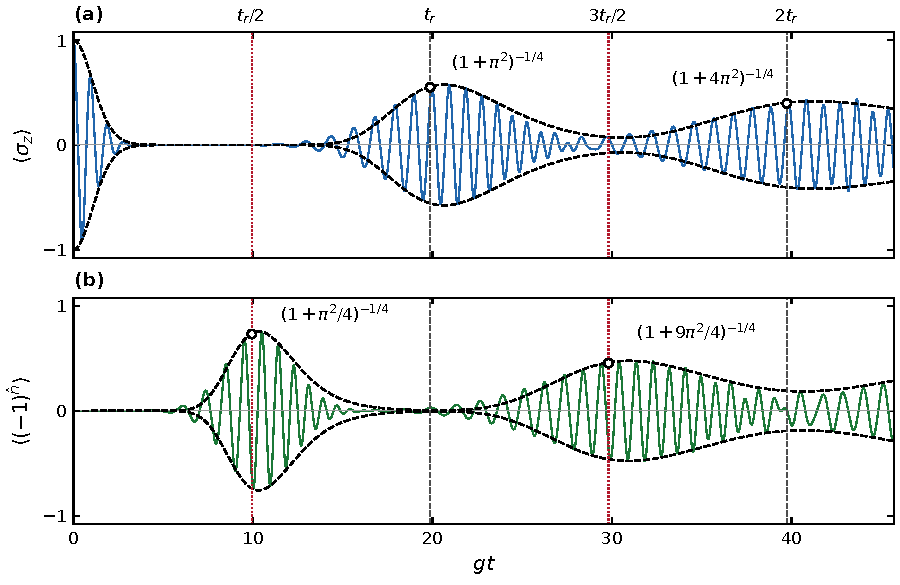
\includegraphics[width=6in]{fig_revival_envelopes.pdf}
\caption{(a) Atomic inversion and (b) photon-number parity for $\nbar = 10$ from the exact solution (solid), with the envelopes of Eq.~(\ref{eq:envelope}) (dashed), evaluated as in Sec.~S1 of the Supplemental Material with $\nbar+1$ kept in the phases. The bumps are centered at $2\pi k\sqrt{\nbar+1}/g$, slightly after $kt_r$, with integer $k$ for the inversion and half-odd-integer $k$ for the parity. Vertical lines mark multiples of $t_r/2$. Circles mark the closed-form amplitudes $(1+\pi^2k^2)^{-1/4}$ at $t = kt_r$. The inversion revives when the two field components coincide; the parity revives when they are opposite each other, which is when the cat state exists.}
\label{fig:envelopes}
\end{figure*}

\textit{The half revival is a revival of the parity.} By Eq.~(\ref{eq:overlaps}) the parity is the overlap of one component with the reflection of the other. The two are opposite each other when $\varphi = (k+\tfrac12)\pi$, so the parity is negligible except near odd multiples of $t_r/2$, where it follows Eq.~(\ref{eq:envelope}) with $k$ replaced by $k+\tfrac{1}{2}$ [Fig.~\ref{fig:envelopes}(b)]. Its amplitude at $t_r/2$ is $(1+\pi^2/4)^{-1/4} = 0.733$; an ideal superposition of two coherent states would give unity~\cite{assemat2019}. Under that envelope the parity oscillates at the Rabi frequency $2g\sqrt{\nbar}$, and at the instant $t = t_r/2$,
\begin{equation}
\begin{aligned}
\langle(-1)^{\hat{n}}\rangle_{t_r/2} &\simeq -\,\frac{\cos(\pi\nbar-\eta)}{(1+\pi^2/4)^{1/4}},\\
\eta &= \tfrac{1}{2}\arctan\frac{\pi}{2} = 0.502,
\end{aligned}
\label{eq:parity}
\end{equation}
which is $-0.642$ for even integer $\nbar$ and $+0.642$ for odd. Without the shear this is the $-\cos\pi\nbar$ of Ref.~\cite{assemat2019}; the shear reduces the amplitude to 0.733 and shifts the phase by $\eta$. The comb of odd or even photon numbers seen in simulations~\cite{buzek1992}, and the parity oscillations of Refs.~\cite{knight2024, birrittella2015, assemat2019}, are both manifestations of this quantity: whether the cat state is ``odd'' or ``even'' is not a property of the model but a matter of the Rabi phase at the instant of observation.

\textit{Cat fidelity, squeezing, and negativity.} At $t_r/2$ the shear is $s = \pi/2$. The squared overlap of a sheared component with a coherent state is $[\det(V(s)+\tfrac12 I)]^{-1/2} = (1+s^2/4)^{-1/2}$, which is the peak value of the $Q$ function given in Ref.~\cite{gea-banacloche1991}. The fidelity of the field with the best superposition of two coherent states therefore tends, as $\nbar\to\infty$, to
\begin{equation}
F_{\rm cat} = (1+\pi^2/16)^{-1/2} = 0.786,
\label{eq:fidelity}
\end{equation}
a limit that contains no $\nbar$. The half-revival state is commonly written as a superposition of two coherent states that becomes more accurate as the field grows~\cite{larson2021}. The disentanglement does become exact as $\nbar\to\infty$ (Sec.~\ref{sec:next}), but the components do not become coherent states: a larger field does not make a better cat state, because the shear accumulated by half the revival time is the same in vacuum units. Each component is squeezed by $\sinh r = \pi/4$, a noise reduction of 6.3~dB in its best quadrature; this is the result of Ref.~\cite{gea-banacloche1991} evaluated at $t_r/2$, and Ref.~\cite{woods1993} gives the time up to which the squeezing survives. Finally, the interference term of the Wigner function of two Gaussians of different shape is spread over a larger area than that of two identical ones; integrating its modulus (Sec.~S1 of the Supplemental Material) gives
\begin{equation}
\delta = \frac{2}{\pi}\,(1+s^2)^{1/4} = \frac{2}{\pi}\,(1+\pi^2/4)^{1/4} = 0.869,
\label{eq:negativity}
\end{equation}
against $2/\pi = 0.637$ for an ideal cat state~\cite{kenfack2004}. The half-revival state is a poorer copy of the ideal cat state and at the same time more non-classical by this measure, and for the same reason.

The revival height, the parity amplitude, and the cat fidelity are values of one function. Define $Z_k \equiv \bra{\Phi_-}e^{-2\pi ik\hat{n}}\ket{\Phi_+}$ at the time $t = kt_r$, so that $\mathrm{Re}\,Z_k$ is the inversion for integer $k$ and the parity for half-odd-integer $k$. Equation~(\ref{eq:lemma}) gives $|Z_k| \simeq |G(k)|$ with
\begin{equation}
G(k) = (1+i\pi k)^{-1/2},
\label{eq:G}
\end{equation}
and the three are $|G(1)|$, $|G(\tfrac12)|$, and $|G(\tfrac14)|^2$. Equation~(\ref{eq:parity}) is $\mathrm{Re}\,Z_{1/2}$, with $\arg G(\tfrac12) = -\eta$ and the prefactor of Eq.~(\ref{eq:nextorder}).

\section{Next order: corrections of order $1/\nbar$}
\label{sec:next}

The cubic term of Eq.~(\ref{eq:expansion}), the skewness of the Poisson distribution, and the difference between $n$ and $n+1$ are all of relative order $\nbar^{-1/2}$. They are odd in $\delta n$, so at the revival times their first-order effect on $Z_k$ vanishes and the leading correction is of order $1/\nbar$. Carrying the expansion through (Sec.~S2 of the Supplemental Material) we find
\begin{equation}
\begin{aligned}
Z_k &= e^{2\pi ik(\nbar+1)}\,G(k)\left[1 + \frac{j(k)}{\nbar} + O(\nbar^{-2})\right],\\
j(k) &= -\frac{K(8K^2+3)}{96\,(K-i)^3},\qquad K = \pi k.
\end{aligned}
\label{eq:nextorder}
\end{equation}
For $k = \tfrac12$ this gives $j = 0.0075-0.0571i$ and reproduces the exact parity at $t_r/2$ for $\nbar = 10$, $-0.6408$, to within $10^{-4}$.

The same order controls how completely the atom and field disentangle. Equation~(\ref{eq:twobranch}) assumed that shifting $n$ by one changes the phase by the same amount $\varphi$ for every $n$; in fact the change is $\varphi\sqrt{\nbar/n}$, so the atomic state paired with each field component varies slightly across the photon-number distribution. Keeping this variation, and the difference between $c_n$ and $c_{n+1}$, turns Eq.~(\ref{eq:skeleton}) into (Sec.~S2 of the Supplemental Material)
\begin{equation}
\mathcal{P}(t) = 1 - \tfrac{1}{2}\cos^2\varphi - \frac{(1+\varphi^2)\sin^2\varphi + \varphi\sin\varphi\cos\varphi}{8\nbar},
\label{eq:purity}
\end{equation}
valid between the collapse and the revival. The leading term and the part of the correction proportional to $\varphi^2\sin^2\varphi$ follow from the Gaussian loss of purity found by Gea-Banacloche~\cite{gea-banacloche1992} and from the Bloch vector of Ref.~\cite{kennedy2010}; the remaining terms are of the same order and are needed for the constant in Eq.~(\ref{eq:residual}). At half the revival time
\begin{equation}
\begin{aligned}
\mathcal{P}(t_r/2) &= 1 - \frac{4+\pi^2}{32\,\nbar},\\
S(t_r/2) &\simeq h\!\left(\frac{4+\pi^2}{64\,\nbar}\right).
\end{aligned}
\label{eq:residual}
\end{equation}
At finite $\nbar$ the disentanglement is never complete; the residual entropy falls only as $(\log\nbar)/\nbar$, which is why it is still 0.14~bit at $\nbar = 10$ and 0.02~bit at $\nbar = 100$. Figure~\ref{fig:portrait} shows that Eq.~(\ref{eq:purity}) follows the exact curves closely even at $\nbar = 10$.

\begin{figure*}[t]
\centering
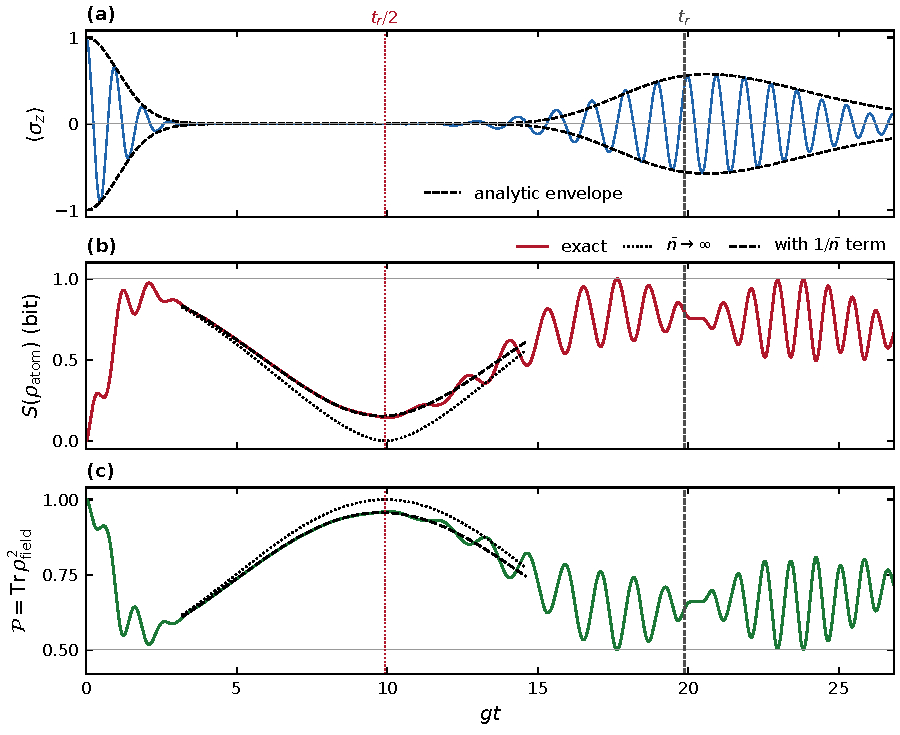
\includegraphics[width=6in]{fig_portrait_model.pdf}
\caption{One collapse--revival cycle for $\nbar = 10$: (a) atomic inversion with the envelope of Eq.~(\ref{eq:envelope}), evaluated as in Fig.~\ref{fig:envelopes}; (b) entanglement entropy of the atom; (c) purity of the reduced field. Solid lines are exact. Between collapse and revival, dotted lines are the first-order result, Eq.~(\ref{eq:skeleton}), and dashed lines include the $1/\nbar$ term of Eq.~(\ref{eq:purity}). Vertical lines mark $t_r/2$ (dotted) and $t_r$ (dashed); gray horizontal lines mark $S = 1$~bit and $\mathcal{P} = 1/2$.}
\label{fig:portrait}
\end{figure*}

\section{Numerical tests, and what limits them}
\label{sec:numerics}

\subsection{Testing the closed forms}

Because Eq.~(\ref{eq:exact}) is exact, the closed forms can be tested without solving a differential equation: the sums over $n$ are evaluated directly, with the Poisson weights truncated where they fall below $10^{-30}$. Table~\ref{tab:test} and Fig.~\ref{fig:convergence} show the result. For $|Z_1|$, $|Z_{1/2}|$, the parity, and $F_{\rm cat}$ the relative error of the leading term falls as $1/\nbar$ from $\nbar\approx 20$--$40$ onwards, as Sec.~\ref{sec:next} requires. The scaled impurity $\nbar(1-\mathcal{P})$ and the negativity approach their limits non-monotonically (their errors change sign near $\nbar\approx 30$ and 75) and reach the $1/\nbar$ law only for $\nbar$ of several hundred. With the correction $j(k)/\nbar$ the error of $Z_k$ falls as $1/\nbar^2$: at $\nbar = 100$ the parity amplitude is reproduced to seven digits. The cat fidelity in Table~\ref{tab:test} is the maximum of $\bra{\rm cat}\rho_{\rm field}\ket{\rm cat}$ over the amplitude $\beta$ and the relative phase $\theta$ of a cat state proportional to $\ket{\beta}+e^{i\theta}\ket{{-}\beta}$; if the two coherent amplitudes and their weights are left free the maximum is slightly larger (0.802, 0.793, and 0.788 for $\nbar = 10$, 25, and 100) and approaches the same limit from above. The negativity is computed by the Fourier method of Sec.~S3 of the Supplemental Material, which reaches $\nbar$ of several thousand ($\delta = 0.86864$ at $\nbar = 6400$, against the limit 0.86872).

\begin{table*}[t]
\caption{Closed forms for $\nbar\to\infty$ against the exact state. $|Z_1|$ and $|Z_{1/2}|$ are the amplitudes of the inversion at $t_r$ and of the parity at $t_r/2$; the other entries are evaluated at $t_r/2$. For the parity the upper sign of the limit applies to even $\nbar$. For the entropy the value of the formula is given in parentheses.}
\label{tab:test}
\begin{ruledtabular}
\begin{tabular}{llcccc}
Quantity & Closed form & Limit & $\nbar = 10$ & $\nbar = 25$ & $\nbar = 100$ \\
\hline
Revival height $|Z_1|$ & $(1+\pi^2)^{-1/4}$ & 0.5507 & 0.5496 & 0.5498 & 0.5505 \\
Parity amplitude $|Z_{1/2}|$ & $(1+\pi^2/4)^{-1/4}$ & 0.7328 & 0.7333 & 0.7330 & 0.7329 \\
Parity & Eq.~(\ref{eq:parity}) & $\mp0.6424$ & $-0.6408$ & $+0.6418$ & $-0.6423$ \\
Cat fidelity $F_{\rm cat}$ & $(1+\pi^2/16)^{-1/2}$ & 0.7864 & 0.7805 & 0.7841 & 0.7859 \\
Negativity $\delta$ & $(2/\pi)(1+\pi^2/4)^{1/4}$ & 0.8687 & 0.8505 & 0.8805 & 0.8672 \\
Scaled impurity $\nbar(1-\mathcal{P})$ & $(4+\pi^2)/32$ & 0.4334 & 0.4023 & 0.4335 & 0.4335 \\
Entropy $S$ (bit) & Eq.~(\ref{eq:residual}) & 0 & 0.144 (0.151) & 0.072 (0.072) & 0.022 (0.022) \\
\end{tabular}
\end{ruledtabular}
\end{table*}

\begin{figure*}[t]
\centering
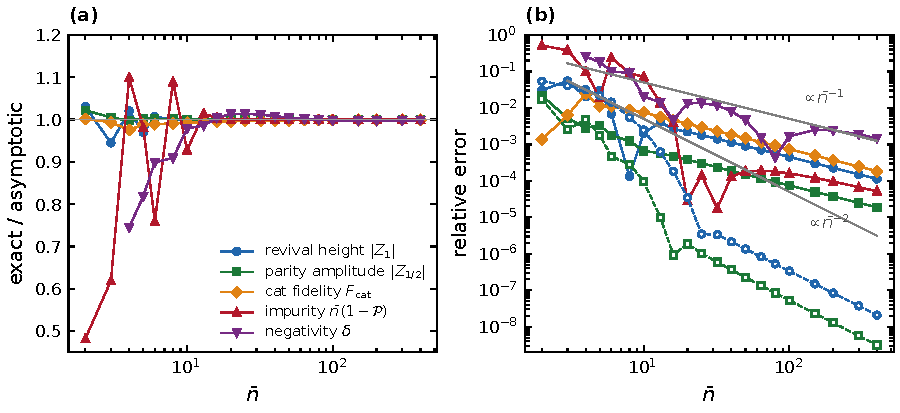
\includegraphics[width=6in]{fig_convergence.pdf}
\caption{Convergence of the closed forms of Table~\ref{tab:test} for $\nbar$ from 2 to 400. (a) Exact value divided by its $\nbar\to\infty$ limit. (b) Relative error. Filled symbols: leading term; open symbols and dashed lines: $|Z_1|$ and $|Z_{1/2}|$ with the $1/\nbar$ correction of Eq.~(\ref{eq:nextorder}). The gray lines have slopes $-1$ and $-2$.}
\label{fig:convergence}
\end{figure*}

\subsection{Where the expansion fails}

Four limits are visible (Sec.~S4 of the Supplemental Material). First, for $\nbar\lesssim 5$ the picture does not apply: the collapse and the first revival overlap, the inversion at $t_r/2$ is not zero, and quantities such as the scaled impurity are off by tens of percent [Fig.~\ref{fig:convergence}(a)]; the scaled impurity is still 7\% off at $\nbar = 10$. Second, the bumps of Eq.~(\ref{eq:envelope}) widen with $k$ while their spacing stays fixed, so successive revivals merge once $k$ is of order $\sqrt{\nbar}/2$; for $\nbar = 10$ the first and second already overlap [Fig.~\ref{fig:envelopes}(a)]. The components also become steadily less Gaussian: a phase that is a function of $\hat n$ moves points along arcs of the circle rather than along its tangent, which bends the components at relative order $\nbar^{-1/2}$ even for a purely quadratic phase, and the cubic term of Eq.~(\ref{eq:expansion}), of relative size $\varphi/8\sqrt{\nbar}$, adds to this. Third, the constants converge at very different speeds. The cat fidelity is within 1\% of its limit at $\nbar = 10$, but the squeezing of a single component is only 3.6~dB there, 5.9~dB at $\nbar = 100$, and 6.2~dB at $\nbar = 400$, against the limit 6.3~dB: a variance is far more sensitive than an overlap to the bending of the component along the circle (Fig.~\ref{fig:wigner}), consistent with the finding that the squeezing survives only up to times of order $\nbar^{3/4}/g$~\cite{woods1993}. Fourth, agreement at the center of a revival does not imply agreement elsewhere: on the flanks of a bump the envelope is accurate only to relative order $\nbar^{-1/2}$ (for $\nbar = 100$, at one standard deviation from the center, 3\% in the form used for the figures and 6\% for Eq.~(\ref{eq:envelope}) as written), and so is the phase of the fast oscillation.

\subsection{Limits of the numerics}

When the model is extended, for example to include loss, a closed-form solution is no longer available and one integrates the Schr\"{o}dinger or master equation. We use QuTiP~\cite{johansson2012, johansson2013, lambert2026}; Eq.~(\ref{eq:exact}) then becomes the standard against which the numerical method is calibrated. Section~S3 of the Supplemental Material does this in detail, and four findings are worth recording.

(i) \emph{Truncation.} With the field truncated to $N_{\rm cav}$ Fock states the error of the entropy at $t_r/2$ follows the Poisson weight left outside to within an order of magnitude: $10^{-2}$ at $N_{\rm cav} = 20$, $4\times10^{-7}$ at 30, for $\nbar = 10$. A thermal field with the same $\nbar$ needs $N_{\rm cav} = 150$ and a squeezed vacuum about 250 for a weight of $10^{-6}$; a fixed $N_{\rm cav}$ silently changes the physics.
(ii) \emph{Integrator.} With QuTiP's default tolerances the inversion for $\nbar = 10$ is accurate to $4\times10^{-5}$ over one and a half revival times, and the error scales with the relative tolerance; the default is adequate for every figure here and inadequate for testing a $1/\nbar^2$ law.
(iii) \emph{Phase-space sampling.} The fringes of the cat have period $\pi/\sqrt{2\nbar}$. At exactly two grid points per fringe the negativity is wrong by 0.16; errors of $7\times10^{-3}$ persist up to four points per fringe and of $10^{-3}$ up to ten. Because $|W|$ has kinks, the error decreases only as the inverse square of the number of points per fringe, and erratically.
(iv) \emph{Time sampling.} A trace sampled at about two points per Rabi period shows a plausible but spurious envelope. The entropy oscillates at twice the Rabi frequency and needs twice the sampling.

Computational cost limits the accessible $\nbar$. The exact sums cost a time proportional to $\nbar$. A Wigner function on a grid that resolves the fringes over the whole circle needs of order $\nbar^2$ points, and a master-equation run to $t_r/2$ a time of order $\nbar^{3}$, which is why our study of loss stops at $\nbar = 25$ while the unitary tests reach $\nbar = 6400$.

\section{Cavity loss}
\label{sec:loss}

The picture extends to the question of how long the cat state survives, analyzed by Gea-Banacloche~\cite{gea-banacloche1993} and by Meunier \textit{et al.}~\cite{meunier2006}; what follows is a short route to their result. Photon loss at rate $\kappa$, described by the master equation $\dot\rho = -i[H,\rho]/\hbar + \kappa(a\rho a^\dagger - \tfrac12\{a^\dagger a,\rho\})$, destroys the coherence between two coherent states $\ket{\beta_1}$, $\ket{\beta_2}$ at the rate $\tfrac12\kappa|\beta_1-\beta_2|^2$~\cite{walls1985, haroche2006}. The two components are a distance $2\sqrt{\nbar}\sin\varphi$ apart in amplitude, so the rate is $2\kappa\nbar\sin^2\varphi$~\cite{auffeves2003}: zero at first, and $2\kappa\nbar$ only when the cat state is fully formed. Its integral up to the angle $\varphi$, $(2\kappa\nbar^{3/2}/g)(\varphi-\tfrac12\sin2\varphi)$, is the exponent obtained in Ref.~\cite{meunier2006}; at $t_r/2$ it gives the visibility of the fringes,
\begin{equation}
\frac{\delta(\kappa)}{\delta(0)} \simeq \exp\!\left(-\frac{\pi\kappa\,\nbar^{3/2}}{g}\right),
\label{eq:visibility}
\end{equation}
where $\delta(\kappa)$ is the negativity at $t_r/2$ for the loss rate $\kappa$ and $\delta_0\equiv\delta(0)$. Using the final rate $2\kappa\nbar$ throughout, a tempting simplification, doubles the exponent. Equation~(\ref{eq:visibility}) implies that the largest tolerable loss falls as $\nbar^{-3/2}$: asking for $\delta > 0.05$ requires $\kappa/g < \ln(\delta_0/0.05)/(\pi\nbar^{3/2}) \approx 0.9\,\nbar^{-3/2}$.

Figure~\ref{fig:loss} tests this against master-equation simulations for $\nbar$ from 2 to 25. Plotted against $\pi\kappa\nbar^{3/2}/g$ the data for different $\nbar$ fall on one curve, which follows Eq.~(\ref{eq:visibility}) down to $\delta/\delta_0\approx 0.2$. For $\nbar = 10$ and $\kappa/g = 0.02$ the prediction is 0.14 and the simulation gives 0.17. Beyond that the estimate fails systematically: at small $\nbar$ the negativity falls faster, and at large $\nbar$ more slowly, than predicted. The estimate neglects two things (Secs.~S2 and S5 of the Supplemental Material). The loss shrinks the amplitude, so the components rotate faster and are no longer opposite each other at the nominal $t_r/2$; and at finite $\nbar$ part of the negativity of the lossless state resides in the non-Gaussian distortion of the components themselves rather than in the fringes. The simulated threshold loss rate $\kappa_c$, at which $\delta = 0.05$, is $\kappa_c/g = 0.033$ at $\nbar = 10$; for $12\leq\nbar\leq25$, $\kappa_c\nbar^{3/2}/g = 1.15\pm0.03$, that is, the predicted exponent with a prefactor about 25\% above the estimate.

\begin{figure*}[t]
\centering
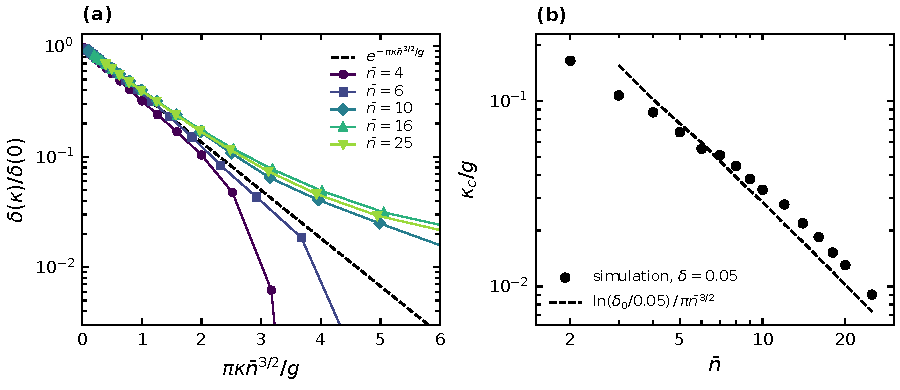
\includegraphics[width=6in]{fig_loss_scaling.pdf}
\caption{Cavity loss. (a) Wigner negativity at $t_r/2$ relative to its lossless value, from master-equation simulations for $\nbar = 4$, 6, 10, 16, and 25, against the scaling variable of Eq.~(\ref{eq:visibility}); dashed line: Eq.~(\ref{eq:visibility}). (b) Threshold loss rate $\kappa_c$ at which $\delta$ falls to 0.05, with the estimate $\ln(\delta_0/0.05)/(\pi\nbar^{3/2})$ (dashed).}
\label{fig:loss}
\end{figure*}

\section{Conclusions}
\label{sec:conclusions}

The collapse and revival of the Jaynes--Cummings model are usually explained with the slope of the Rabi spectrum. Its curvature explains most of what a simulation then shows. To first order the two components of the field rotate; to second order they are sheared by an amount equal to their rotation angle. From the overlap of two sheared Gaussians follow the heights of the revivals and the squeezing of the components, both known since the work of Gea-Banacloche~\cite{gea-banacloche1991}, together with the revival of the parity at half the revival time and the fidelity and negativity of the cat state, each as a closed form independent of $\nbar$. One further order gives the residual atom--field entanglement and the rate at which these limits are approached. Tested against the exact solution, the amplitudes and the fidelity are accurate to about $1/\nbar$, or the amplitudes to $1/\nbar^2$ with the correction term; the formulas fail for small $\nbar$, for late revivals, and for quantities sensitive to the bending of the components. With cavity loss the same picture reproduces the known decay exponent of the cat state~\cite{meunier2006} and its scaling with $\nbar^{3/2}$.

% Keep the two closing sections together: a short block left alone on the last page is set
% in the right-hand column only when REVTeX balances the columns above the reference list.
\vspace{0pt plus 2.6in}\pagebreak[3]\vspace{0pt plus -2.6in}
\begin{acknowledgments}
This work began as a course project in EC 585 and EC 777 at Boston University, taught by Prof.\ Luca Dal Negro.
\end{acknowledgments}

\section*{Data availability}

The code that generates every figure and number in this article, together with the sweep data, is openly available~\cite{nguyen2026code}.

\begin{thebibliography}{99}

\bibitem{jaynes1963}
E.~T.~Jaynes and F.~W.~Cummings, Proc.\ IEEE \textbf{51}, 89 (1963).

\bibitem{eberly1980}
J.~H.~Eberly, N.~B.~Narozhny, and J.~J.~Sanchez-Mondragon, Phys.\ Rev.\ Lett.\ \textbf{44}, 1323 (1980).

\bibitem{gerry2004}
C.~C.~Gerry and P.~L.~Knight, \textit{Introductory Quantum Optics} (Cambridge University Press, Cambridge, 2004).

\bibitem{haroche2006}
S.~Haroche and J.-M.~Raimond, \textit{Exploring the Quantum: Atoms, Cavities, and Photons} (Oxford University Press, Oxford, 2006).

\bibitem{gea-banacloche1990}
J.~Gea-Banacloche, Phys.\ Rev.\ Lett.\ \textbf{65}, 3385 (1990).

\bibitem{gea-banacloche1991}
J.~Gea-Banacloche, Phys.\ Rev.\ A \textbf{44}, 5913 (1991).

\bibitem{buzek1992}
V.~Bu\v{z}ek, H.~Moya-Cessa, P.~L.~Knight, and S.~J.~D.~Phoenix, Phys.\ Rev.\ A \textbf{45}, 8190 (1992).

\bibitem{phoenix1991}
S.~J.~D.~Phoenix and P.~L.~Knight, Phys.\ Rev.\ A \textbf{44}, 6023 (1991).

\bibitem{narozhny1981}
N.~B.~Narozhny, J.~J.~Sanchez-Mondragon, and J.~H.~Eberly, Phys.\ Rev.\ A \textbf{23}, 236 (1981).

\bibitem{fleischhauer1993}
M.~Fleischhauer and W.~P.~Schleich, Phys.\ Rev.\ A \textbf{47}, 4258 (1993).

\bibitem{feranchuk2009}
I.~D.~Feranchuk and A.~V.~Leonov, Phys.\ Lett.\ A \textbf{373}, 517 (2009).

\bibitem{pavlik2024}
S.~I.~Pavlik, Phys.\ Scr.\ \textbf{99}, 015113 (2024).

\bibitem{phoenix1988}
S.~J.~D.~Phoenix and P.~L.~Knight, Ann.\ Phys.\ (N.Y.) \textbf{186}, 381 (1988).

\bibitem{eiselt1991}
J.~Eiselt and H.~Risken, Phys.\ Rev.\ A \textbf{43}, 346 (1991).

\bibitem{larson2021}
J.~Larson and T.~Mavrogordatos, \textit{The Jaynes--Cummings Model and Its Descendants} (IOP Publishing, Bristol, 2021).

\bibitem{knight2024}
P.~L.~Knight, C.~C.~Gerry, R.~J.~Birrittella, and P.~M.~Alsing, J.~Opt.\ Soc.\ Am.\ B \textbf{41}, C91 (2024).

\bibitem{auffeves2003}
A.~Auff\`{e}ves, P.~Maioli, T.~Meunier, S.~Gleyzes, G.~Nogues, M.~Brune, J.~M.~Raimond, and S.~Haroche, Phys.\ Rev.\ Lett.\ \textbf{91}, 230405 (2003).

\bibitem{bild2023}
M.~Bild \textit{et al.}, Science \textbf{380}, 274 (2023).

\bibitem{meystre1982}
P.~Meystre and M.~S.~Zubairy, Phys.\ Lett.\ A \textbf{89}, 390 (1982).

\bibitem{kuklinski1988}
J.~R.~Kukli\'{n}ski and J.~L.~Madajczyk, Phys.\ Rev.\ A \textbf{37}, 3175 (1988).

\bibitem{woods1993}
C.~W.~Woods and J.~Gea-Banacloche, J.~Mod.\ Opt.\ \textbf{40}, 2361 (1993).

\bibitem{gea-banacloche1992}
J.~Gea-Banacloche, Phys.\ Rev.\ A \textbf{46}, 7307 (1992).

\bibitem{kennedy2010}
R.~Kennedy, L.~Horstmeyer, A.~Dragan, and T.~Rudolph, Phys.\ Rev.\ A \textbf{82}, 054302 (2010).

\bibitem{birrittella2015}
R.~Birrittella, K.~Cheng, and C.~C.~Gerry, Opt.\ Commun.\ \textbf{354}, 286 (2015).

\bibitem{assemat2019}
F.~Assemat, D.~Grosso, A.~Signoles, A.~Facon, I.~Dotsenko, S.~Haroche, J.~M.~Raimond, M.~Brune, and S.~Gleyzes, Phys.\ Rev.\ Lett.\ \textbf{123}, 143605 (2019).

\bibitem{gea-banacloche1993}
J.~Gea-Banacloche, Phys.\ Rev.\ A \textbf{47}, 2221 (1993).

\bibitem{meunier2006}
T.~Meunier, A.~Le~Diffon, C.~Ruef, P.~Degiovanni, and J.-M.~Raimond, Phys.\ Rev.\ A \textbf{74}, 033802 (2006).

\bibitem{munhoz2005}
P.~P.~Munhoz and A.~Vidiella-Barranco, J.~Mod.\ Opt.\ \textbf{52}, 1557 (2005).

\bibitem{supplement}
See Supplemental Material at [URL will be inserted by publisher] for the derivations, the numerical methods and their measured errors, the limits of the asymptotic picture, other initial field states, and maps of the cat state under cavity loss.

\bibitem{kenfack2004}
A.~Kenfack and K.~\.{Z}yczkowski, J.~Opt.~B: Quantum Semiclass.\ Opt.\ \textbf{6}, 396 (2004).

\bibitem{johansson2012}
J.~R.~Johansson, P.~D.~Nation, and F.~Nori, Comput.\ Phys.\ Commun.\ \textbf{183}, 1760 (2012).

\bibitem{johansson2013}
J.~R.~Johansson, P.~D.~Nation, and F.~Nori, Comput.\ Phys.\ Commun.\ \textbf{184}, 1234 (2013).

\bibitem{lambert2026}
N.~Lambert \textit{et al.}, Phys.\ Rep.\ \textbf{1153}, 1 (2026).

\bibitem{walls1985}
D.~F.~Walls and G.~J.~Milburn, Phys.\ Rev.\ A \textbf{31}, 2403 (1985).

\bibitem{nguyen2026code}
N.~K.~Nguyen, \textit{QSOL\_CQED}, version 1.2.0, Zenodo (2026), \url{https://doi.org/10.5281/zenodo.24262358}.

\end{thebibliography}

\end{document}
